\part{Referencial teórico}

\chapter[Fundamentação teórica]{Fundamentação teórica}

Este capítulo destina-se a apresentar a fundamentação teórica realizada por meio de revisões da literatura. Seu objetivo é oferecer um catálogo de conceitos que servirá como base para o entendimento do atual trabalho.

\section[Processamento de Linguagem	 Natural]{Processamento de Linguagem Natural}

O Processamento de Linguagem Natural é uma ciência que abranje um conjunto de técnicas e métodos que facilitam a análise e textual por um computador. No atual projeto, técnicas de PLN são aplicadas para extrair as \textit{features} que, por sua vez, serão utilizadas para a realização das classificações. No contexto do aprendizado de máquina, as \textit{features} são as variáveis intrinsecamente presentes nos dados, sendo elas essenciais na identificação de padrões pelo algoritmo.

As técnicas citadas são utilizadas na etapa de extração de atributos, comumente referida como \textit{Feature Extraction}. É a partir dela que se define quais aspectos do texto servirão de insumo para o classificador. Há diversas formas de se abordar a extração de características de um texto, sendo as principais: \textit{Bag-of-Words}, \textit{n-grams}, \textit{Word2Vec} e TF-IDF.

\subsection{Bag-of-Words}

O BoW (\textit{Bag-of-Words}) é um modelo de extração de características de texto bastante flexível, ele descreve o número de ocorrências de palavras de uma frase. Para isso, cada frase é representada por um vetor com n elementos, onde n é o número de palavras do vocabulário. Cada posição representa uma palavra e o elemento é o número de ocorrências daquela palavra na frase. Observe os exemplos a seguir:

\begin{samepage}
(1) “o dia está radiante”

\nopagebreak

(2) “que dia é hoje?”
\end{samepage}

Imagine um vetor para cada uma dessas frases. No BoW, eles seriam semelhantes a estes:

\begin{center}
\begin{table}[htbp]
\centering
\begin{tabular}{c|ccccccc}
 & \textbf{o} & \textbf{dia} & \textbf{está} & \textbf{radiante} & \textbf{que} & \textbf{é} & \textbf{hoje} \\ \hline
\textbf{Vetor 1} & 1 & 1 & 1 & 1 & 0 & 0 & 0 \\
\textbf{Vetor 2} & 0 & 1 & 0 & 0 & 1 & 1 & 1 
\end{tabular}
\caption{Exemplo de \textit{Bag-of-Words}}
\label{bow}
\end{table}
\end{center}

Como é possível observar na Tabela \ref{bow}, com apenas duas pequenas frases, o vocabulário é bastante limitado, apenas sete palavras, porém, o que é mais comum em situações reais são vocabulários absurdamente grandes, o que resulta em vetores igualmente grandes e com quase todos os seus elementos iguais a 0.

Outro fator que vale ser notado é que a ordem das palavras não são levadas em consideração neste modelo, apenas a existência delas.

\subsection{N-grams}

O modelo \textit{n-grams} é bastante similar ao \textit{Bag-of-Words} no sentido de definir um vetor para a frase e realizar uma contagem de ocorrências. A diferença está na \textit{vetorização}, que se dá por um processo diferente. Ao invés de representar palavras do vocabulário nas posições do vetor, o \textit{n-grams} propõe uma representação por \textit{substrings}  com um número \textit{N} de palavras. Desta forma, este modelo se torna mais adequado para capturar nuances do texto (CITAR: Lundborg, 2017 Master Thesis), onde a ordem das palavras é relevante e não apenas a presença delas. Utilizando as frases do exemplo anterior, observe como os vetores ficariam para \textit{N = 2}.

\begin{samepage}
(1) “o dia está radiante”

\nopagebreak

(2) “que dia é hoje?”
\end{samepage}

\begin{center}
\begin{table}[htbp]
\centering
\begin{tabular}{c|cccccc}
 & \textbf{o dia} & \textbf{dia está} & \textbf{está radiante} & \textbf{que dia} & \textbf{dia é} & \textbf{é hoje} \\ \hline
\textbf{Vetor 1} & 1 & 1 & 1 & 0 & 0 & 0 \\
\textbf{Vetor 2} & 0 & 0 & 0 & 1 & 1 & 1
\end{tabular}
\caption{Exemplo de \textit{n-grams}}
\label{ngrams}
\end{table}
\end{center}

\subsection{TF-IDF}

Em algumas situações, apenas avaliar a frequência de termos pode não ser o ideal. A forma com que a língua é estruturada favorece a dominância de uma série de termos dos quais não carregam a em si conteúdo significativo para a realização de classificações (CITAR: Brownlee, Jason).

A fim de reduzir o grau de relevância desses termos que predominam a linguagem naturais, temos o modelo \textit{TF-IDF}, que significa \textit{Term Frequency-Inverse Document Frequency}, onde:

\begin{itemize}
\item \textit{Term Frequency}: Do inglês, significa frequência do termo dentro da frase atual. No caso, termo pode ser uma palavra ou múltiplas, como no modelo N-grams.
\item \textit{Inverse Document Frequency}: Trata-se de um valor inverso à frequência em que o termo é encontrado nas frases do conjunto de dados como um todo.
\end{itemize}

Para calcular o \textit{TF-IDF}, utiliza-se a seguinte fórmula:

\begin{equation}
w_{i,j} = tf_{i,j}\times\log \frac{N}{df_i}
\end{equation}

Observe que, ao aplicar esta fórmula obtém-se um valor que é mais alto quando o termo for frequente no texto analisado, porém, raro em todos os textos, ou seja, as particularidades de cada texto são acentuadas.

\subsection{Limpeza do Texto}

Parte do pré-processamento do texto é a realização de sua limpeza. Para tal, foram utilizadas duas técnicas:

\begin{itemize}
\item \textbf{\textit{Stemização}}: Do inglês, \textit{stemming}, refere-se ao processo de reduzir as palavras à uma forma primitiva, como um radical. Este processo visa garantir que pequenas variações de uma mesma palavra seja interpretada pelo computador como uma palavra só. Dessa forma, além de economizar recursos, pois o computador precisará processar um vetor de menor dimensão, também beneficiará o classificador considerar que palavras com pequenas variações de gênero ou número carregam em si o mesmo sentido. Como em “\textit{historiador}” e “\textit{historiadoras}”, que ficariam apenas “\textit{histori}”, por exemplo.

\item \textbf{Remoção das \textit{stop words}}: As \textit{stop words} (palavras vazias) são palavras que agregam pouco ou nenhum valor semântico que deva ser levado em consideração pelo classificador. Geralmente, são as palavras mais comuns da língua, incluindo artigos, preposições, verbos de ligação, entre outras. Não existe um conjunto bem definido de quais palavras devem ser classificadas como palavras vazias, e, naturalmente, esse conjunto depende do idioma em questão. Para o atual projeto, foi utilizado o conjunto em português do \textbf{NLTK}.
\end{itemize}

\section{Aprendizado de máquina}

Visando a construção de um classificador textual que seja capaz de identificar pequenos textos que caracterizam discurso de ódio e facilitar o trabalho de moderação de comentários, a aprendizagem de máquina se apresenta como uma possível solução. Aprendizado de máquina pode ser definido como uma forma de Inteligência Artificial (IA) que permite que um sistema aprenda através de dados ao invés de uma programação explícita. \cite{mlfordummyes:2018}

Os primeiros passos na área do Aprendizado de Máquina aconteceram em 1943, quando, ao tentar explicar como o cérebro funciona, um neurofisiologista e um matemático construíram, utilizando circuitos elétricos, a primeira rede neural \cite{nnhistory}. No contexto da processamento de linguagem natural, suas aplicações são diversas, como: predição de palavras (como em teclados de smartphones), chatbots e classificação de textos. Esta última, pode ser definida como o objetivo principal deste trabalho.
No atual contexto, ao utilizar do aprendizado de máquina para a classificação de textos, podemos automatizar e evoluir um modelo, de modo a tornar a intervenção humana seja mínima ou nula no processo de moderação de comentários.

\section{Classificação}

Os modelos de Aprendizado de Máquina costumam ser divididos em 2 tipos: Supervisionado, do qual um conjunto de dados previamente rotulado serve de insumo, o modelo analisa estes dados e tem como objetivo prever futuros rótulos para novos dados, e o Não-Supervisionado, onde o modelo busca encontrar padrões ou estruturas intrínsecas nos dados de treino \cite{mwmachinelearning}. Observe a imagem abaixo.

\begin{figure}[!htb]
    \center{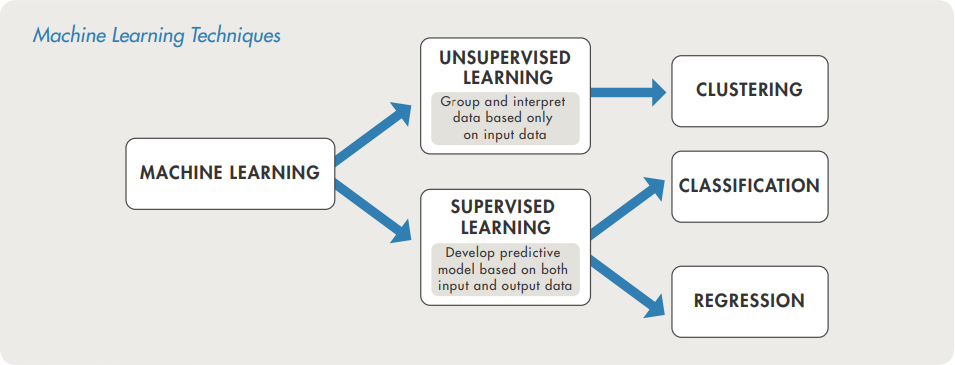
\includegraphics[width=\textwidth]
    {figuras/ml_techniques.png}}
    \caption{\label{fig:my-label} Diagrama sobre tipos de aprendizado de máquina}
\end{figure}

A escolha de qual tipo de AM deve ser utilizado depende da natureza do problema que está sendo abordado e dos dados disponíveis. No atual trabalho, serão utilizados modelos de classificação, que são do tipo de Aprendizado Supervisionado. Estes modelos estão detalhados a seguir.

\subsection{Support Vector Machines}

O termo Support Vector Machines engloba um conjunto de modelos que buscam classificar os dados em 2 classes diferentes. Para tal, as features são analisadas e inseridas em um plano com N-1 features de dimensão, de modo que se forme uma “linha” que divide as 2 classes na maior margem possível entre elas. Essa linha é formada com o auxílio dos dois pontos mais próximos de cada classe. Através delas, duas linhas de suporte são traçadas, e a divisão principal é formada. Daí vem o nome “support vector”.

\begin{figure}[!htb]
    \center{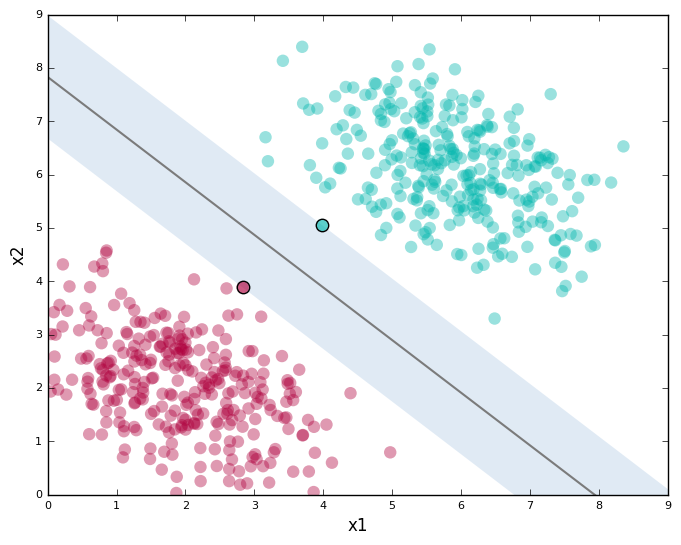
\includegraphics[scale=0.3]
    {figuras/svm_example.png}}
    \caption{\label{fig:my-label} Diagrama SVM para 2 features}
\end{figure}

O primeiro modelo que utiliza de vetores de suporte é o modelo Gradiente Descendente Estocástico, ou SDG (Stochastic Gradient Descent). Diferente de alguns modelos de vetores de suporte que, para realizar uma atualização de parâmetro necessita computar todas as features, o SDG faz uma iteração mais leve, de modo que apenas um ou um grupo de features é verificado a cada atualização. Desse modo, é possível trabalhar com um número alto de features e/ou exemplos de treino \cite{scikit-learn}.

O outro modelo baseado nesse princípio, é o Vetor de Suporte-C, ou SVC, implementado pela libsvm \cite{libsvm}. Esse modelo segue a ideia padrão de computar todas as features a cada atualização. Seu diferencial está num parâmetro, chamado parâmetro C. Quanto maior o valor desse parâmetro, menores as margens da linha de divisão serão, de modo que todos os pontos sejam classificados corretamente. Caso o valor seja pequeno, a linha de divisão busca por margens maiores, mesmo que algumas amostras sejam classificadas incorretamente.

Em nosso modelo de treinamento, o SVC foi utilizado em conjunto do TF-IDF, de modo que se defina várias features para o funcionamento correto do algoritmo. Contudo, o melhor valor para a variável C foi de 4.0, considerado bem alto. Por causa desse valor, é possível presumir que a linha que classifica as frases fica bem próxima do limite de ambas, uma vez que uma margem grande, alcançada através de um C pequena, não é desejado para a maior performance.

\begin{figure}[!htb]
    \center{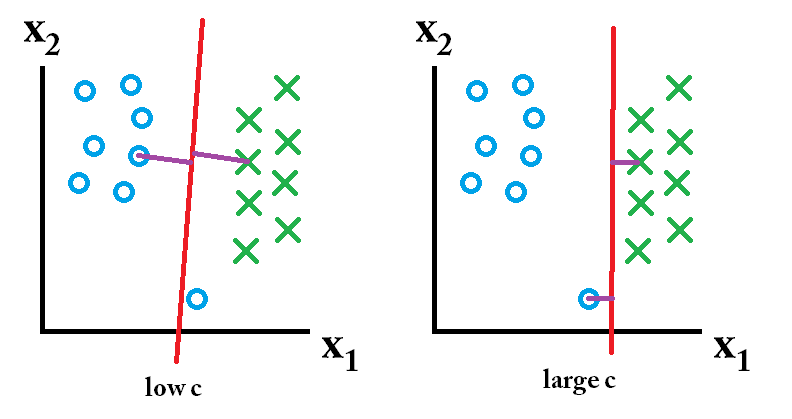
\includegraphics[scale=0.3]
    {figuras/svm_example2.png}}
    \caption{\label{fig:my-label} Diagrama representando as mudanças da variável C}
\end{figure}

\subsection{Decision Tree/Random Forest}

Árvores de decisão é um modelo usado tanto para regressão, quanto para classificação \cite{decision-tree}. São fáceis de serem interpretadas, justamente por se tratar de um modelo baseado em uma estrutura de dados em que estamos acostumados a lidar. Além disso, o modelo suporta classificação numérica ou categórica, e consegue obter um desempenho por qualidade muito bom com relação a outros modelos de classificação, independente do tamanho do dataset \cite{performance-comparison}. Contudo, por se tratar de um algoritmo guloso, alguns problemas podem ser vistos nos resultados, como o sobreajuste, ou “overfitting”. O overfitting define um modelo estático que se adequa muito bem a um conjunto de dados já conhecido, mas que não consegue prever novos resultados caso um conjunto de dados diferente seja apresentado. Esse caso piora mais e mais, proporcionalmente igual à profundidade da árvore.  Com o objetivo de resolver isso, criou-se o modelo de Floresta randômica. O “Random forest” consiste em um combinado de árvores de decisão, onde o resultado de cada uma é unido, com o objetivo de encontrar uma predição mais estável e preciso.

Em nosso modelo de treinamento do algoritmo de Random forest, utilizamos um ‘n-gram’ de 1 a 4 palavras, de modo que as árvores possam crescer, dada a quantidade de features fornecida. A profundidade das árvores não foi limitada, mas foi definido um total de 100 árvores. Desse modo, mesmo que as árvores alcancem uma alta profundidade, o “overfitting” dos resultados não ocorre.

\subsection{Naive Bayes/Multinomial NB}
O modelo de Naive Bayes é baseado no teorema probabilístico de Bayes, e tem como forte premissa de que as “features”, ou palavras de cada sentença, são fortemente independentes. Utilizando do teorema, uma tabela de probabilidades é criada, utilizando a frequência de ocorrência das palavras. Para criação de tal tabela, o TF-IDF é uma das opções para a extração dessas features. A partir dessa tabela, o classificador de Naive Bayes analisa as palavras, de acordo com a probabilidade da feature ser “positiva” ou “negativa”, caso seja utilizado para se analisar o sentimento de uma frase, por exemplo.

O Multinomial Naive Bayes é uma extensão do modelo de Naive Bayes, mas com a utilização da distribuição multinomial para cada feature. Desse modo, o modelo Multinomial NB funciona bem para dados que podem ser contados, se tornando um bom modelo para classificação de tópicos, por exemplo \cite{russel-ia}.

Em nosso modelo de treinamento, tanto o modelo tradicional quanto o multinomial funcionam melhor com o dataset isento de stop words, pois a alta frequência das mesmas pode atrapalhar a eficiência do algoritmo. O n-gram que gerou o melhor resultado foi com apenas uma palavra. Isso pode ser explicado pelo fato de que frases que contém discurso de ódio são caracterizadas por palavras específicas, raramente utilizadas.

\subsection{MLP}

O MLP, ou Perceptron de múltiplas camadas, é um modelo de treinamento que tem como base a simulação do raciocínio humano. Seu funcionamento mais básico consiste em ao menos 3 camadas: A camada de entrada (onde as features serão passadas), a camada oculta (onde os cálculos são realizados), e a camada de saída. As camadas são compostas por neurônios, que realizam o cálculo utilizando de informações passadas pelos neurônios das camadas anteriores. Num MLP, podem haver várias camadas ocultas, dependendo do tipo de problema a ser resolvido. Cada camada oculta busca transformar o valor da camada anterior, utilizando da soma linear dos pesos e de uma função de ativação não linear, como a função tangente hiperbólica. Ao chegar na última camada oculta, a camada de saída recebe seu valor e o transforma em valores de saída.

Em nosso modelo de treino, foi utilizado apenas uma camada oculta, contendo 100 neurônios. Este valor busca cobrir casos em que haja muitas features (frases muito grandes podem resultar em altos valores de features), de modo que todas sejam levadas em consideração. Na maioria dos casos, menos de 20 neurônios seriam necessários para classificar a frase corretamente. Além disso, como a escolha é binária, apenas uma camada oculta é necessária, de modo que se crie uma “linha” que classifica a frase.

\begin{figure}[!htb]
    \center{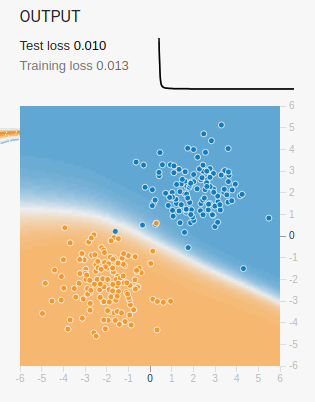
\includegraphics[scale=0.3]
    {figuras/mlp_example.png}}
    \caption{\label{fig:my-label} Diagrama MLP,  4 features de entrada, 1 camada oculta, 8 neurônios}
\end{figure}